\section{方法}\label{sec:method}

DriveCompose 将多视角观测对齐到规范支撑，联合补全潜码，并按指定状态组合解码资产（图~\ref{fig:overview}）。

\begin{figure*}[t]
  \centering
  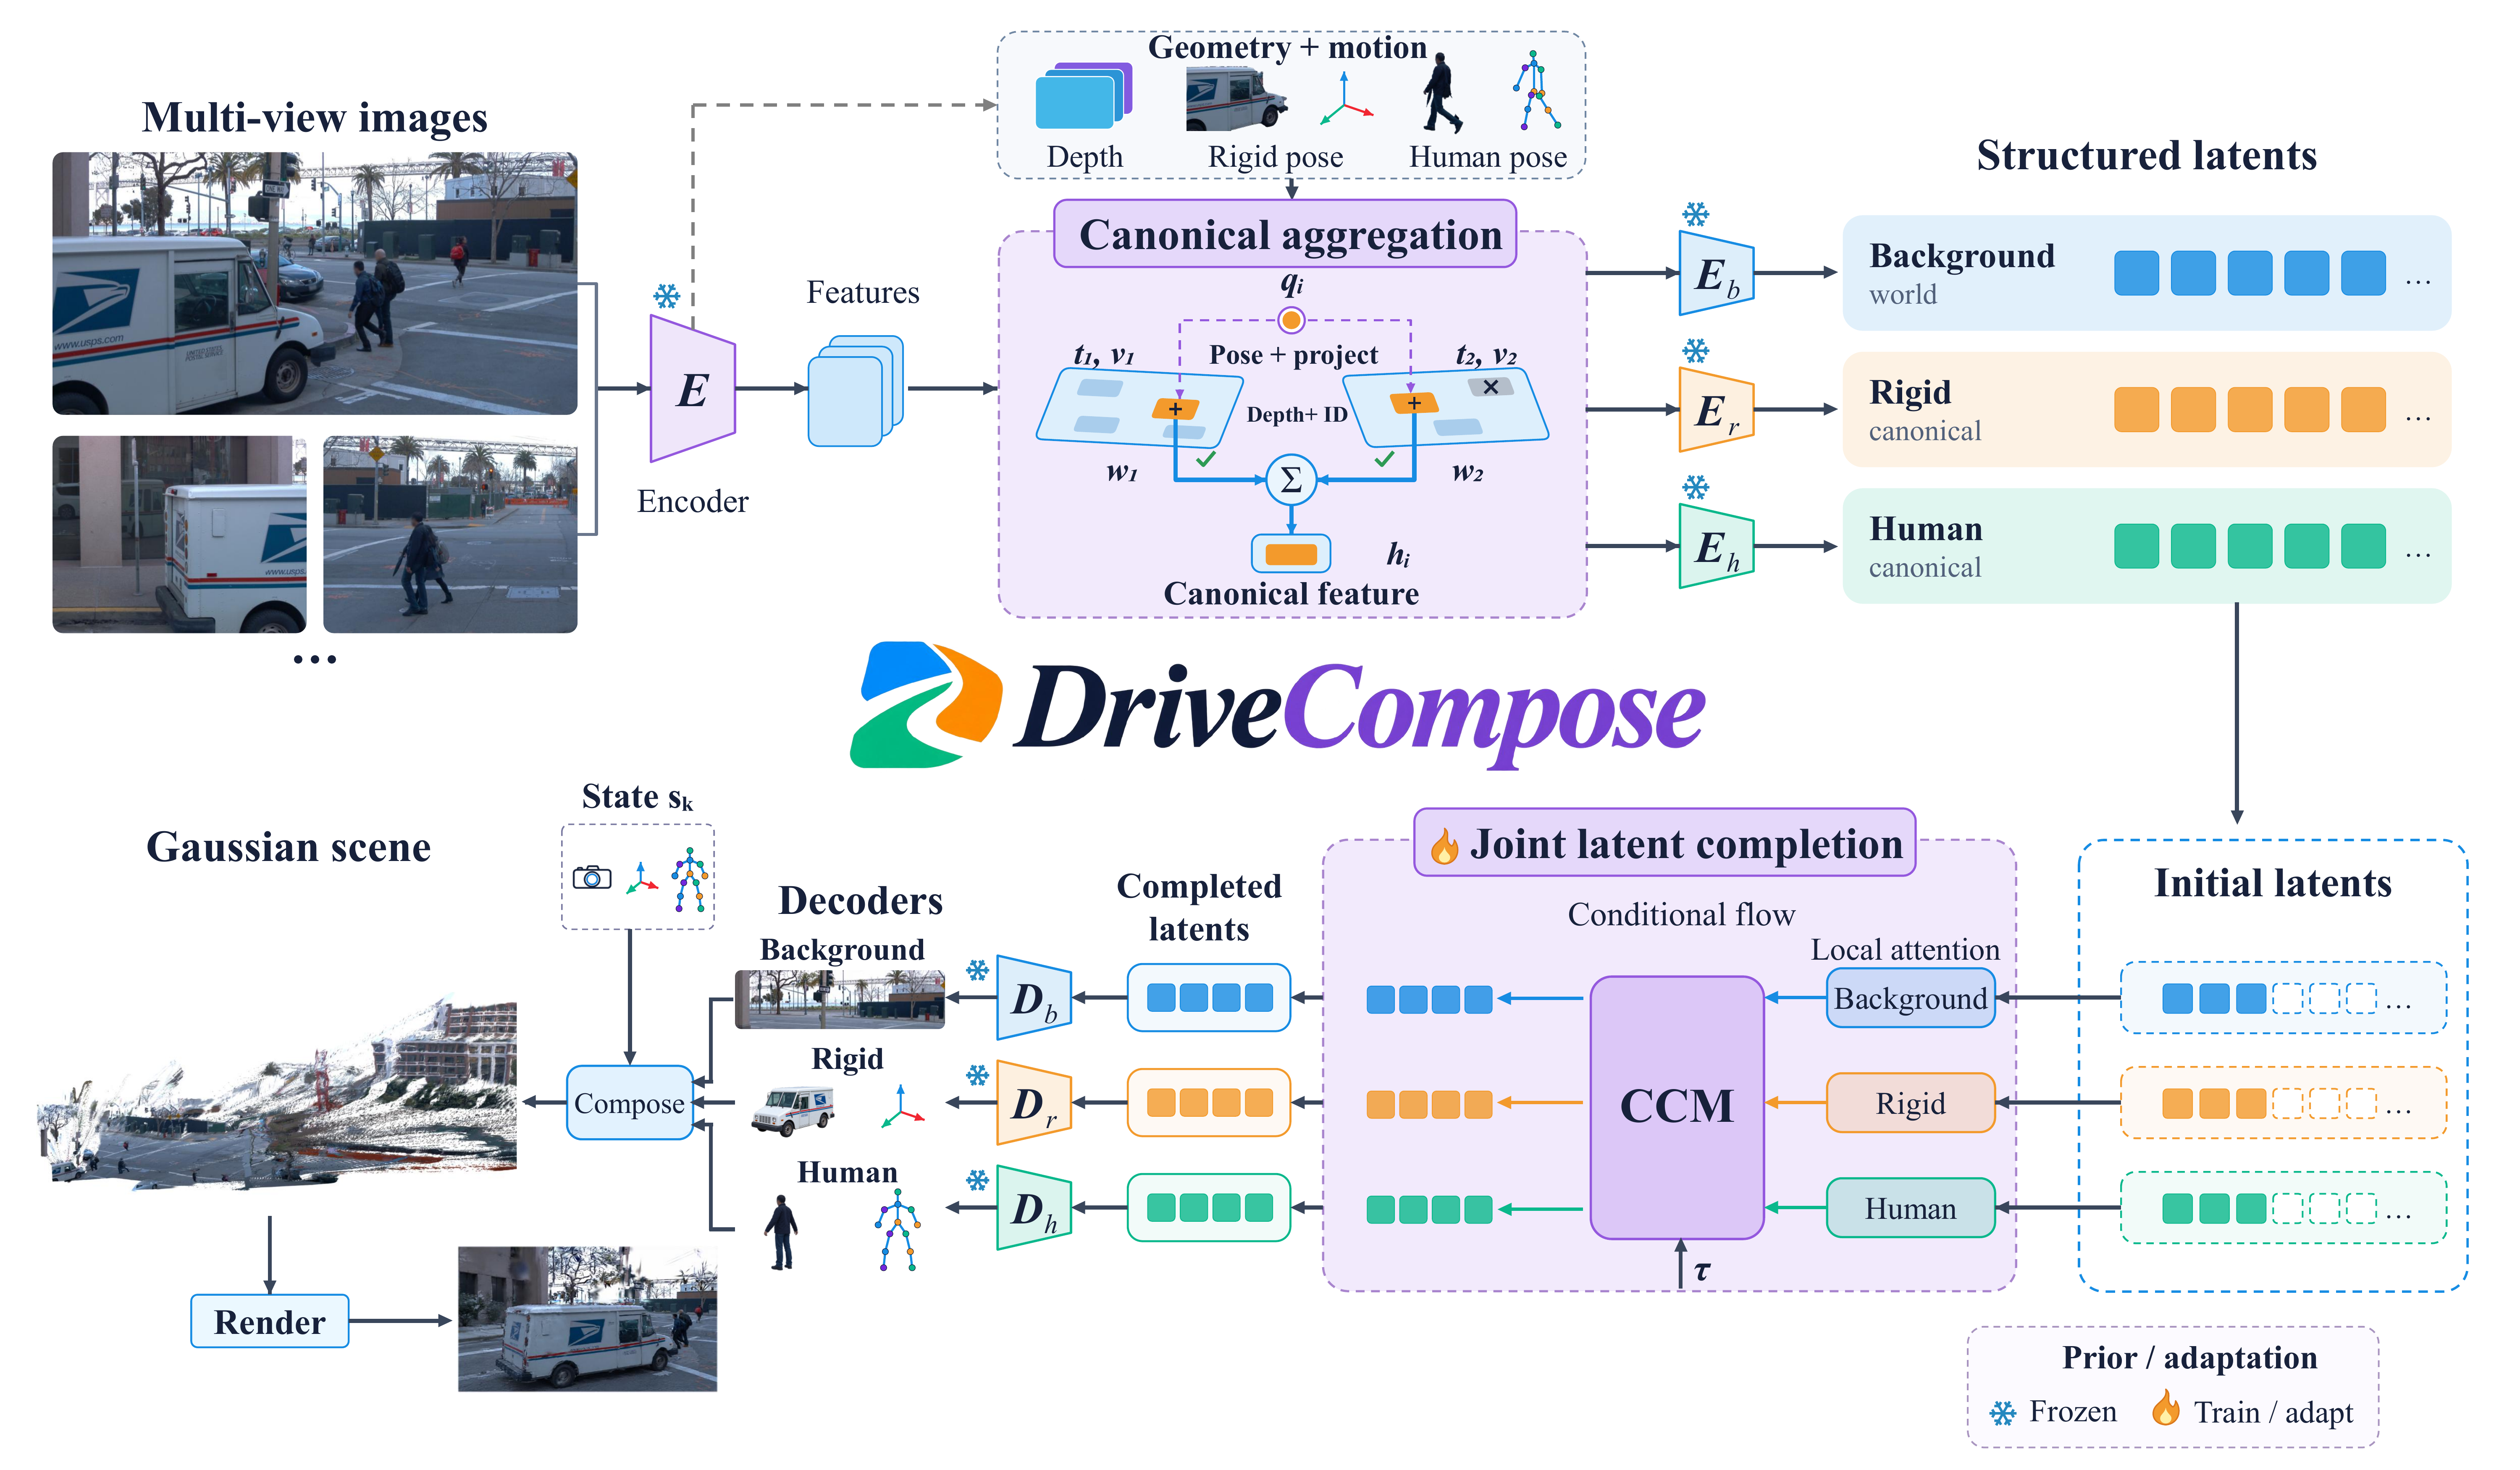
\includegraphics[width=\textwidth]{fig/drivecompose-inference-overview.png}
  \caption{\textbf{DriveCompose 总览。}视觉编码与规范聚合恢复组件特征，类型专属编码器映射结构化潜码，联合补全和高斯解码生成背景、车辆与人体，用于状态驱动组合。场景与资产画面均为机制示意。}
  \label{fig:overview}
\end{figure*}

\subsection{问题定义与可组合表示}
\label{sec:representation}

输入是同步图像日志 $\mathbf I_{t,v}$、时间戳、相机内参及相机到传感器支架的标定。受控评价给定支架位姿、实例身份、车辆框与根轨迹，以及目标人体关节。人体体型与绑定由上下文恢复，重建不使用目标 RGB 或测试 LiDAR。坐标约定与图像预处理见补充材料附录 D。

输出为可组合高斯场景

\begin{equation}
\mathcal W=\bigl(\mathcal G_b,C_{\rm sky},V_{\rm sky},
\{\mathcal A_a\},\mathcal B,\xi\bigr),
\label{eq:world}
\end{equation}

其中，$\mathcal G_b$ 是世界空间背景，$C_{\rm sky}$ 是天空立方体贴图，$V_{\rm sky}$ 表示其有效方向，$\mathcal A_a$ 是身份 $a$ 对应的规范资产，$\mathcal B$ 是有限空间支撑，$\xi$ 是采样种子。这些组件通过高斯泼溅渲染~\cite{kerbl2023gaussians}。车辆表示为局部几何与尺寸固定的刚体资产，人体另存静止骨架和蒙皮权重。场景状态控制这些固定组件的放置与关节运动。

我们通过条件生成建模缺失内容。令 $\mathcal Q$ 为恢复得到的查询布局，$C$ 为其观测证据。补全模型采样未知潜码 $\mathbf z_u$，编解码器 $D_\psi$ 将组合后的潜码解码为场景内容：

\begin{equation}
\mathbf z_u\sim p_\theta(\mathbf z_u\mid C,\mathcal Q),
\qquad
\mathcal W=D_\psi(\mathbf z^{\rm obs},\mathbf z_u;\mathcal Q).
\label{eq:generative-reconstruction}
\end{equation}

查询布局为每个潜码指定空间位置和所属组件。补全在这一布局中生成未知潜码，解码后仍保留其组件身份与运动绑定。

\subsection{视觉恢复与规范聚合}
\label{sec:visual-encoding}

Driving Log Encoder 从各图像提取 patch 特征，并在相机与时间戳之间交换池化上下文~\cite{dosovitskiy2021vit,vaswani2017attention}。几何预测头输出相机光轴深度、法线、置信度、语义和实例归属，将图像特征关联到三维表面及其所属组件。轨迹级身份槽将持久身份、尺寸和人体体型与逐帧变化的根位姿、关节旋转分开表示。网络结构与状态参数化细节见补充材料附录 D。

\label{sec:queries}

\paragraph{空间支撑。}

每个查询存储规范位置 $\mathbf q_i$、单元尺度 $\boldsymbol\delta_i$、类型 $k_i$、局部注意力组 $g_i$ 和参考世界坐标 $\mathbf q_i^w$。可靠深度样本提供表面锚点。背景锚点与有限世界网格结合；刚体锚点经逆 SE(3) 变换对齐后，与局部包围体中的网格结合。人体查询位于规范模板表面，天空查询为按立方体贴图面分组的单位方向。这些支撑为已见与缺失内容提供明确位置。

固定布局以规范坐标标识组件内容，以第一帧世界坐标 $\mathbf q_i^w$（包括人体蒙皮）联系组件与周围场景。

\paragraph{运动感知证据聚合。}

对于每份观测，我们将规范查询放到对应的资产状态：

\begin{equation}
\mathbf p_i(t)=
\begin{cases}
\mathbf q_i,& k_i=\mathrm{background},\\
\operatorname{xyz}(\mathbf T^w_a(t)\bar{\mathbf q}_i),& k_i=\mathrm{rigid},\\
\operatorname{xyz}(\mathbf T^w_h(t)\mathbf A_i(t)\bar{\mathbf q}_i),& k_i=\mathrm{human}.
\end{cases}
\label{eq:query-placement}
\end{equation}

其中，$\bar{\mathbf q}_i$ 为齐次坐标，$\operatorname{xyz}$ 提取欧氏坐标，$\mathbf A_i(t)$ 为加权蒙皮变换。投影得到查询深度 $z_{i,t,v}$，并采样图像特征 $\boldsymbol\phi_{i,t,v}$、深度 $d_{i,t,v}$ 和置信度 $c_{i,t,v}$，按置信度及归一化深度残差 $r=(d-z)/(\eta_{\rm abs}+\eta_{\rm rel}d)$ 为观测赋权。指示量 $a_{i,t,v}$ 选择同一实例中可见且深度一致的观测（附录 D）：

\begin{align}
w_{i,t,v}&=a_{i,t,v}c_{i,t,v}\exp(-r_{i,t,v}^2/2),\\
\mathbf h_i&=\frac{\sum_{t,v}w_{i,t,v}[\boldsymbol\phi_{i,t,v};r_{i,t,v}]}
{\max(\varepsilon,\sum_{t,v}w_{i,t,v})}.
\label{eq:aggregation}
\end{align}

掩码 $m_i$、$f_i$ 和 $u_i$ 区分已见表面、射线标记的自由空间和未知内容，满足 $m_i+f_i+u_i=1$。置信度取有效观测的最大值，两份可靠深度射线票确定自由空间标签。天空特征依据相机旋转和天空语义，按观察方向聚合。判定式与投影足迹掩码审计见附录 D。

\subsection{潜表示编码}
\label{sec:codec}

类型专属编码器将 129 维聚合特征及空间支撑 $[\mathbf h_i;\mathbf q_i;\boldsymbol\delta_i]$ 输入带 LayerNorm 的 $135\!\rightarrow\!128\!\rightarrow\!128$ MLP，得到 $D=128$ 维潜码，并保留查询类型、归属和坐标系。部分与完整分支共享此映射，掩码和置信度单独作为补全条件。未观测潜码置零，已见码记为 $\mathbf z^{\rm obs}$。

\subsection{联合潜空间补全}
\label{sec:completion}

\begin{figure}[t]
  \centering
  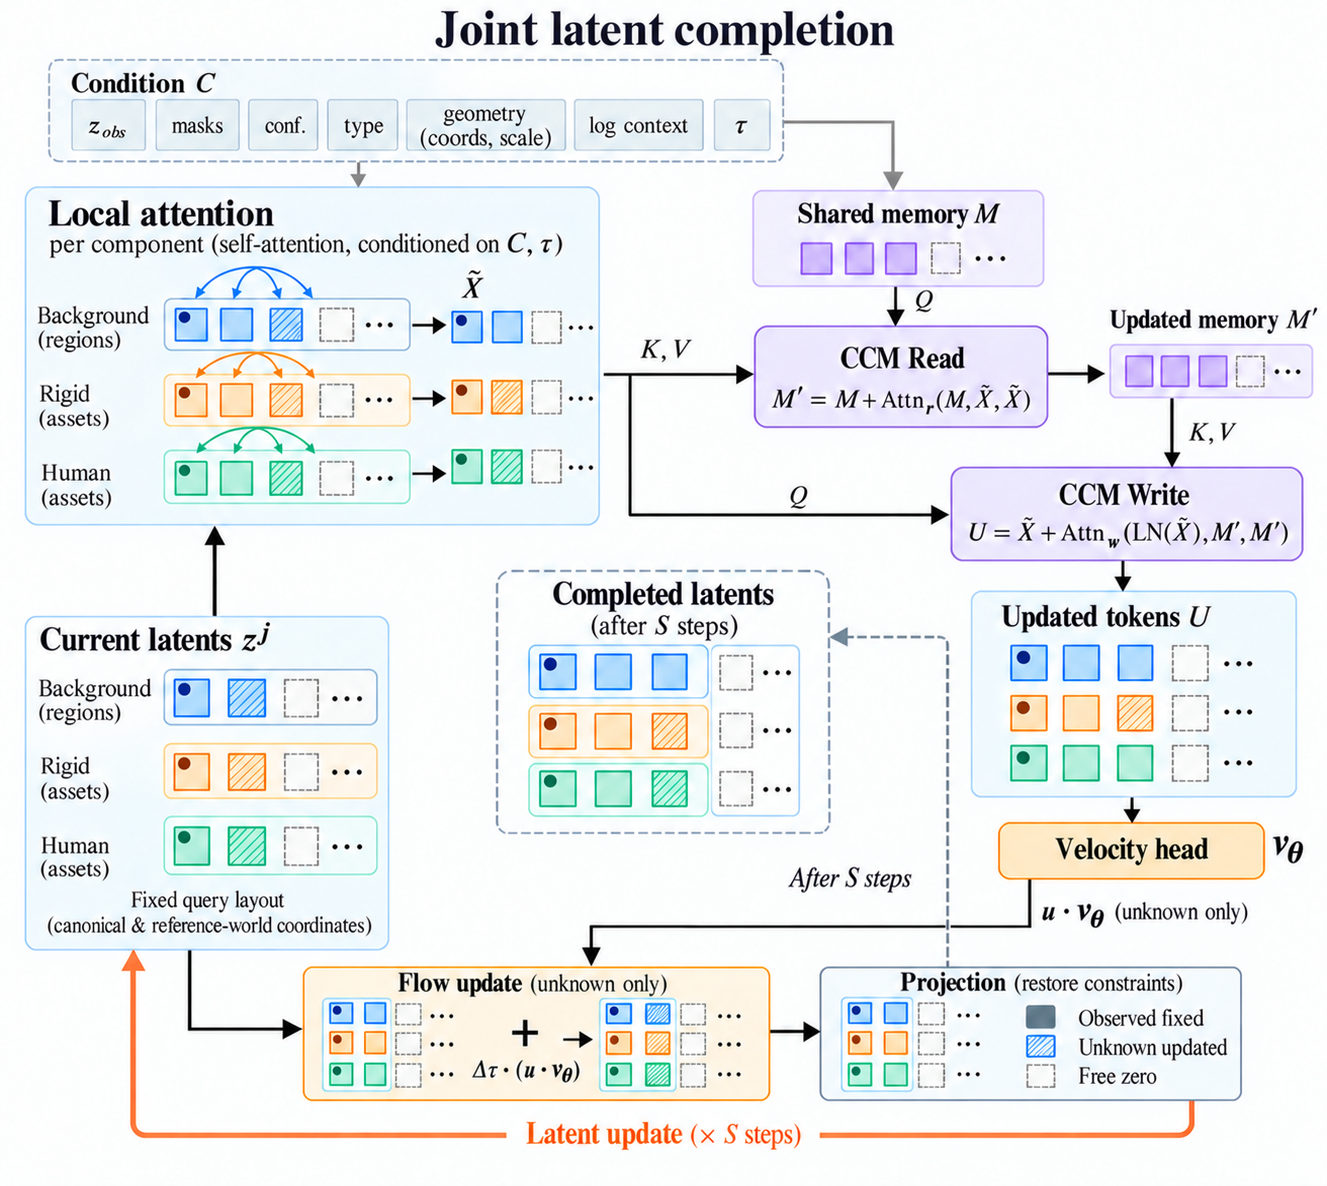
\includegraphics[width=\linewidth]{fig/drivecompose-joint-completion.png}
  \caption{\textbf{联合潜空间补全。}CCM 读入局部特征并回写共享上下文，投影约束流更新只改变未知码。附录 L 提供放大图。}
  \label{fig:joint-completion}
\end{figure}

\paragraph{生成式补全模块。}

生成式补全模块（Generative Completion Module，GCM）由场景条件流 Transformer 与约束采样组成（图~\ref{fig:joint-completion}）。我们采用 DiT 风格的 Transformer~\cite{peebles2023dit} 参数化补全速度场，并通过流匹配训练~\cite{lipman2022flowmatching}。输入结合当前潜码、已见潜码、掩码、置信度、类型、两种坐标描述、单元尺度和池化日志特征。背景按空间邻域分组，每个资产构成一个局部组，天空方向按立方体贴图面分组。局部自注意力分别处理各组，跨组件记忆模块（Cross-Component Memory，CCM）随后通过共享记忆交换上下文：

\begin{align}
\mathbf M'&=\mathbf M+\operatorname{Attn}_{r}
(\mathbf M,\widetilde{\mathbf X},\widetilde{\mathbf X}),\\
\mathbf U&=\widetilde{\mathbf X}+\operatorname{Attn}_{w}
(\operatorname{LN}(\widetilde{\mathbf X}),\mathbf M',\mathbf M').
\label{eq:memory-exchange}
\end{align}

其中，$\widetilde{\mathbf X}$ 拼接局部 token，注意力参数依次为查询、键和值。$\mathbf U$ 后接残差前馈更新。流时间调制局部归一化，记忆由可学习 token 与日志摘要初始化。

\paragraph{流训练与约束采样。}

令 $\mathbf z_1$ 为同一查询布局上的完整目标，$\boldsymbol\epsilon\sim\mathcal N(0,\mathbf I)$ 为高斯噪声。在流时间 $\tau\in[0,1]$，我们仅对未知内容插值：

\begin{equation}
\mathbf z_\tau=m\odot\mathbf z^{\rm obs}
+u\odot[(1-\tau)\boldsymbol\epsilon+\tau\mathbf z_1].
\label{eq:flow-path}
\end{equation}

已见潜码固定，自由空间潜码保持为零。未知查询的目标速度为 $\mathbf z_1-\boldsymbol\epsilon$。引入可选损失选择器 $s_i$，目标为

\begin{equation}
\mathcal L_{\rm flow}=
\frac{\sum_i u_i s_i\|\mathbf v_\theta(\mathbf z_\tau,\tau,C)_i
-(\mathbf z_{1,i}-\boldsymbol\epsilon_i)\|_2^2}
{D\max(1,\sum_i u_i s_i)}.
\label{eq:flow-loss}
\end{equation}

先验学习使用全部未知查询均具有有效目标的样本，$s_i$ 在这些目标中选择损失项（第~\ref{sec:training} 节）。

推理时，以噪声初始化未知潜码，并执行 $S$ 次 Euler 步，步长为 $\Delta\tau=1/S$：

\begin{equation}
\mathbf z^{j+1}=\Pi_{m,f}\!\left[
\mathbf z^j+\Delta\tau\,u\odot
\mathbf v_\theta(\mathbf z^j,j/S,C)\right].
\label{eq:sampling}
\end{equation}

每步后 $\Pi_{m,f}$ 恢复已见潜码、清零自由空间潜码。种子确定一次补全，解码一次后跨状态复用。

\subsection{分类型高斯解码}
\label{sec:decoding}

背景、刚体和人体高斯解码器分别将每个查询独立映射为中心位于其支撑单元内的 $K=4$ 个子高斯。人体子高斯继承查询的蒙皮权重；刚体子高斯共用所属资产的刚体变换。不透明度乘以 $1-f_i$，使自由空间查询不能产生可见高斯。独立天空头在观测支持的方向域 $V_{\rm sky}$ 内预测立方体贴图颜色。高斯与外观参数化详见补充材料附录 E。

各查询独立解码。冻结编解码器并保留已见潜码，使已见高斯参数保持不变。自由射线损失约束新增高斯对可见性与透明度混合的影响，第~\ref{sec:observation-preservation} 节给出实测。

\subsection{场景组合}
\label{sec:composition}

\paragraph{状态驱动渲染。}

时刻 $k$ 的状态 $s_k$ 指定自车位姿、活动资产、刚体变换，以及人体根位姿与关节姿态。刚体位姿对规范高斯的中心和协方差施加刚体变换，人体关节姿态通过存储的蒙皮权重使高斯变形，补全表面因此随相应身体部位运动。具体变换见补充材料附录 C。渲染器合成背景、活动资产和有效天空：

\begin{equation}
o_k=\mathcal R(\operatorname{Compose}(\mathcal W,s_k),\mathcal C_k).
\label{eq:simulation}
\end{equation}

背景与规范资产保持固定，新相机及参与者状态复用同一份完成内容。

\subsection{训练流程}
\label{sec:training}
训练依次进行视觉恢复、潜表示拟合、补全先验学习和通过渲染适配。部分输入固定 $\mathcal Q$，包括单元尺度、组件归属及人体绑定。完整网格提供各单元内的表面样本，多视图渲染与冻结视觉编码器得到 $\mathbf h_i^{\rm full}$，再由共享的类型专属编码器映射为 $\mathbf z_{1,i}=E_{k_i}([\mathbf h_i^{\rm full};\mathbf q_i;\boldsymbol\delta_i])$。无表面单元采用零特征和不透明度监督。

潜表示拟合结束后，恢复模块和 codec 保持冻结。阶段三使用每个未知查询均具有完整目标的合成样本；阶段四仅更新 GCM，以 $1{:}3$ 混合完整合成样本和 740 条真实训练日志。四阶段共更新 287,360 步，目标构造、网络规模和训练设置详见附录 B。
